%%%%%%%%%%%%%%%%%%%%%%%%%%%%%%%%%%%%%%%%%%%%%%%%%%%%%%%%%%%%%%%%%%%%%%%%%%%%%%%%
%Tutorial slides on Python.
%
% Author: FOSSEE
% Copyright (c) 2009-2016, FOSSEE, IIT Bombay
%%%%%%%%%%%%%%%%%%%%%%%%%%%%%%%%%%%%%%%%%%%%%%%%%%%%%%%%%%%%%%%%%%%%%%%%%%%%%%%%

\documentclass[14pt,compress]{beamer}

% Modified from: generic-ornate-15min-45min.de.tex
\mode<presentation>
{
  \usetheme{Warsaw}
  \useoutertheme{infolines}
  \setbeamercovered{transparent}
}

\usepackage[english]{babel}
\usepackage[latin1]{inputenc}
%\usepackage{times}
\usepackage[T1]{fontenc}

% Taken from Fernando's slides.
\usepackage{ae,aecompl}
\usepackage{mathpazo,courier,euler}
\usepackage[scaled=.95]{helvet}

\definecolor{darkgreen}{rgb}{0,0.5,0}

\usepackage{listings}
\lstset{language=Python,
    basicstyle=\ttfamily\bfseries,
    commentstyle=\color{red}\itshape,
  stringstyle=\color{darkgreen},
  showstringspaces=false,
  keywordstyle=\color{blue}\bfseries}

%%%%%%%%%%%%%%%%%%%%%%%%%%%%%%%%%%%%%%%%%%%%%%%%%%%%%%%%%%%%%%%%%%%%%%
% Macros
\setbeamercolor{emphbar}{bg=blue!20, fg=black}
\newcommand{\emphbar}[1]
{\begin{beamercolorbox}[rounded=true]{emphbar}
      {#1}
 \end{beamercolorbox}
}
\newcounter{time}
\setcounter{time}{0}
\newcommand{\inctime}[1]{\addtocounter{time}{#1}{\tiny \thetime\ m}}

\newcommand{\typ}[1]{\lstinline{#1}}

\newcommand{\kwrd}[1]{ \texttt{\textbf{\color{blue}{#1}}}  }

%%% This is from Fernando's setup.
% \usepackage{color}
% \definecolor{orange}{cmyk}{0,0.4,0.8,0.2}
% % Use and configure listings package for nicely formatted code
% \usepackage{listings}
% \lstset{
%    language=Python,
%    basicstyle=\small\ttfamily,
%    commentstyle=\ttfamily\color{blue},
%    stringstyle=\ttfamily\color{orange},
%    showstringspaces=false,
%    breaklines=true,
%    postbreak = \space\dots
% }

%%%%%%%%%%%%%%%%%%%%%%%%%%%%%%%%%%%%%%%%%%%%%%%%%%%%%%%%%%%%%%%%%%%%%%
% Title page
\title[Saving scripts]{Introductory Scientific Computing with
Python}
\subtitle{Saving scripts}

\author[FOSSEE] {FOSSEE}

\institute[IIT Bombay] {Department of Aerospace Engineering\\IIT Bombay}
\date[] {Mumbai, India
}
%%%%%%%%%%%%%%%%%%%%%%%%%%%%%%%%%%%%%%%%%%%%%%%%%%%%%%%%%%%%%%%%%%%%%%

%\pgfdeclareimage[height=0.75cm]{iitmlogo}{iitmlogo}
%\logo{\pgfuseimage{iitmlogo}}


%% Delete this, if you do not want the table of contents to pop up at
%% the beginning of each subsection:
\AtBeginSubsection[]
{
  \begin{frame}<beamer>
    \frametitle{Outline}
    \tableofcontents[currentsection,currentsubsection]
  \end{frame}
}

\AtBeginSection[]
{
  \begin{frame}<beamer>
    \frametitle{Outline}
    \tableofcontents[currentsection,currentsubsection]
  \end{frame}
}

% If you wish to uncover everything in a step-wise fashion, uncomment
% the following command:
%\beamerdefaultoverlayspecification{<+->}

%%\includeonlyframes{current,current1,current2,current3,current4,current5,current6}

%%%%%%%%%%%%%%%%%%%%%%%%%%%%%%%%%%%%%%%%%%%%%%%%%%%%%%%%%%%%%%%%%%%%%%
% DOCUMENT STARTS
\begin{document}

\begin{frame}
  \maketitle
\end{frame}

%% \begin{frame}
%%   \frametitle{Outline}
%%   \tableofcontents
%%   % You might wish to add the option [pausesections]
%% \end{frame}

\section{Exercise}

\begin{frame}[plain,fragile]
\frametitle{Review Problem}
\begin{enumerate}
\item Plot $x, -x, \sin(x), x \sin(x)$ in range $-5\pi$ to $5\pi$
\item Add a legend
\item Annotate the origin
\item Set axes limits to the range of x
\end{enumerate}
\vspace*{-0.15in}
\begin{center}
  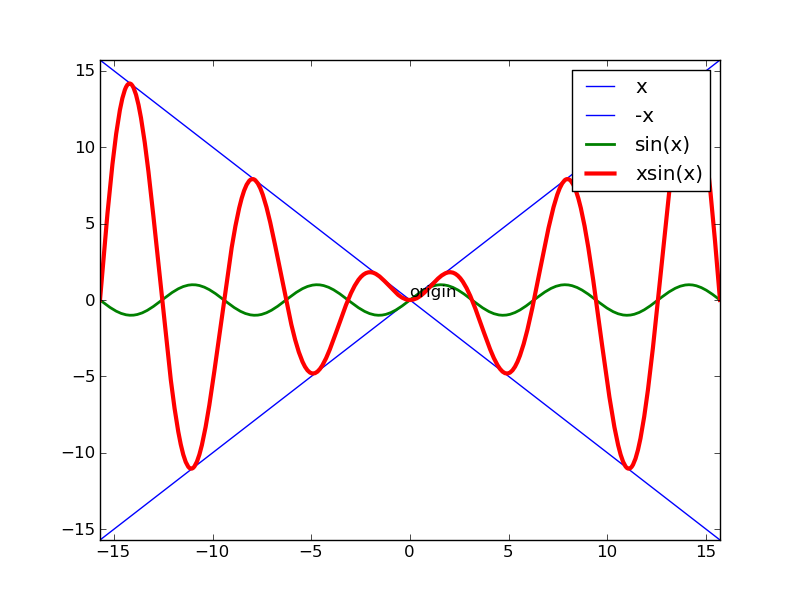
\includegraphics[height=2.6in, interpolate=true]{data/four_plot}
\end{center}
\end{frame}

\begin{frame}[fragile]
\frametitle{Review Problem \ldots}
\alert{Plotting \ldots}
\begin{lstlisting}
In []: x = linspace(-5*pi, 5*pi, 500)
In []: plot(x, x, 'b')
In []: plot(x, -x, 'b')
In []: plot(x, sin(x), 'g', linewidth=2)
In []: plot(x, x*sin(x), 'r',
            linewidth=3)
\end{lstlisting}
$\vdots$
\end{frame}

\begin{frame}[fragile]
\frametitle{Review Problem \ldots}
\alert{Legend \& Annotation\ldots}
\begin{lstlisting}
In []: legend(['x', '-x', 'sin(x)',
               'xsin(x)'])
In []: annotate('origin', xy = (0, 0))
\end{lstlisting}
\alert{Setting Axes limits\ldots}
\begin{lstlisting}
In []: xlim(-5*pi, 5*pi)
In []: ylim(-5*pi, 5*pi)
\end{lstlisting}
\inctime{5}
\end{frame}

\section{Scripts -- Saving \& Running}
\begin{frame}[fragile]
\frametitle{Command History}
Use the \typ{\%hist} \alert{magic} command of IPython
\typ{In []: \%hist}\\
This displays the ``Command History''
\begin{block}{Careful about errors!}
  \kwrd{\%hist} will contain the errors as well.\\
\end{block}
\pause
\begin{block}{Magic Commands?}
  Magic commands are commands provided by IPython to make our life easier.
\end{block}
\end{frame}

\begin{frame}[fragile]
  \frametitle{Saving commands into script}
Use the \typ{\%save} \alert{magic} command of IPython
\begin{block}{}
\typ{\%save script_name line_numbers}
\end{block}
Line numbers specified individually separated by spaces or as a range separated by a dash.\\
\begin{block}{}
\typ{\%save four_plot.py} \alert{\typ{  16 18-27}} \\
\end{block}
Saves from history the commands entered on line numbers \alert{16, 18, 19, 20, \ldots 27}
\end{frame}

\begin{frame}[fragile]
  \frametitle{Saving commands into a script}
  \begin{itemize}
  \item Save lines relevant for the review problem
  \item Hint: example\\ \typ{\%save four_plot.py 16 18-27}
  \item Choose the lines carefully
  \item Edit \typ{four_plot.py} on Spyder
  \item Make sure all the lines are correct
  \item Save the script
  \end{itemize}
\inctime{5}
\end{frame}

\begin{frame}[fragile]
  \frametitle{Creating scripts: alternative}
  \begin{itemize}
  \item Create a new file on Spyder
  \item Copy commands for assignment with your mouse
  \item Save the script to \typ{four_plot.py}
  \end{itemize}
\end{frame}

\begin{frame}[fragile]
  \frametitle{Where is the script saved?}
  \begin{itemize}
  \item \typ{\%save} saves into the current directory
    \vspace*{0.5in}
  \item Use \typ{\%pwd} to print the current directory
  \item Use \typ{\%cd} to change the directory

    \vspace*{0.5in}
  \item Question: how do you find out more about \typ{\%cd}?
  \end{itemize}
\end{frame}


\begin{frame}[fragile]
\frametitle{Python Scripts\ldots}
Now, \typ{four_plot.py} is called a Python Script.
 \begin{itemize}
 \item run the script in IPython using \typ{\%run four_plot.py}\\
 \end{itemize}
\pause
\alert{\typ{NameError: name 'linspace' is not defined}}
\begin{block}{}
To avoid this, run using \alert{\typ{\%run -i four_plot.py}}\\
\end{block}
\pause
Where is the plot?
\begin{lstlisting}
In []: show()
\end{lstlisting}
\end{frame}

\begin{frame}[fragile]
  \frametitle{Exercise}
  \begin{itemize}
  \item Add the \typ{show()} command to \typ{four_plot.py}
  \item Save the file
  \item Test that it works
  \end{itemize}
  \inctime{5}
\end{frame}

\begin{frame}[fragile]
  \frametitle{Result graph}
  \begin{center}
    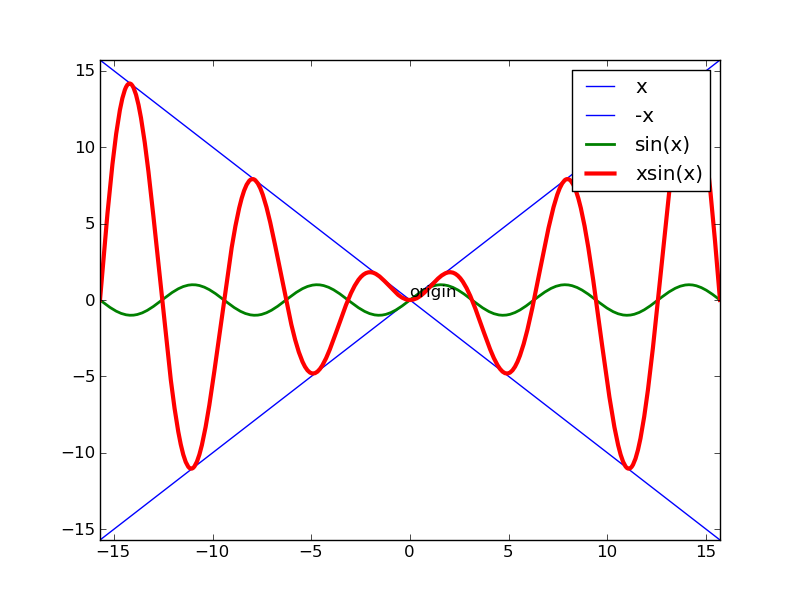
\includegraphics[height=3in, interpolate=true]{data/four_plot}
  \end{center}
\end{frame}

\begin{frame}[fragile]
  \frametitle{Running with Python}
  \begin{itemize}
  \item Start a new terminal
  \item Change directory to where you saved \typ{four_plot.py}
  \item Run the script as:
  \end{itemize}
\begin{lstlisting}
 $ python four_plot.py
\end{lstlisting}
  \pause
  Do you see:
  \begin{small}
\begin{lstlisting}
NameError: name 'linspace' is not defined
\end{lstlisting}
  \end{small}
\end{frame}

\begin{frame}[fragile]
  \frametitle{Imports}
  \begin{itemize}
  \item \typ{ipython --pylab} does magic
  \item Import libraries using \typ{import}
  \end{itemize}
\begin{lstlisting}
In []: from pylab import linspace
\end{lstlisting}
\inctime{5}
\end{frame}

\begin{frame}[fragile]
  \frametitle{Exercise}
  \begin{itemize}
  \item Add \typ{from pylab import linspace} to top of \typ{four_plot.py}
  \item Test that it works
  \end{itemize}
\begin{lstlisting}
# four_plot.py
from pylab import linspace # <-- added
x = linspace(-5*pi, 5*pi, 500)
plot(x, x, 'b')
...
\end{lstlisting}
\end{frame}

\begin{frame}[fragile]
  \frametitle{Try again}
  \begin{itemize}
  \item On terminal
  \item Run the script as:
  \end{itemize}
\begin{lstlisting}
 $ python four_plot.py
\end{lstlisting}
  \pause
  \vspace*{0.15in}
  Do you see:
  \begin{small}
\begin{lstlisting}
NameError: name 'plot' is not defined
\end{lstlisting}
  \end{small}
\end{frame}

\begin{frame}[fragile]
  \frametitle{Exercise}
  \begin{itemize}
  \item Change line 1 to \typ{from pylab import *}
  \item Test that it works
  \end{itemize}
\begin{lstlisting}
# four_plot.py
from pylab import * # <-- added
x = linspace(-5*pi, 5*pi, 500)
plot(x, x, 'b')
...
\end{lstlisting}
\inctime{5}
\end{frame}

\begin{frame}[fragile]
  \frametitle{Solution}
  \small
\begin{lstlisting}
from pylab import *
x = linspace(-5*pi, 5*pi, 500)
plot(x, x, 'b')
plot(x, -x, 'b')
plot(x, sin(x), 'g', linewidth=2)
plot(x, x*sin(x), 'r', linewidth=3)
legend(['x', '-x', 'sin(x)', 'xsin(x)'])
annotate('origin', xy = (0, 0))
xlim(-5*pi, 5*pi)
ylim(-5*pi, 5*pi)
show()
\end{lstlisting}
\end{frame}

\begin{frame}[fragile]
  \frametitle{Note on script file names}
  \begin{itemize}
  \item Should start with a letter
  \item Can use \typ{_} (underscore) and numbers
  \item No \typ{.} allowed
  \item No spaces or special characters
  \end{itemize}
\end{frame}

\begin{frame}[fragile]
  \frametitle{Test}
  \begin{itemize}
  \item \typ{1_script.py}
  \item \typ{script_1.py}
  \item \typ{one11.py}
  \item \typ{one script.py}
  \item \typ{one,script;xxx.py}
  \item \typ{one.two.py}
  \end{itemize}
\end{frame}

\begin{frame}
  \frametitle{Using Spyder and Anaconda}
  \begin{itemize}
  \item Much easier
  \item Write code in the editor
  \item Embedded IPython Console
  \item Save (Ctrl-S or Cmd-S)
  \item Run selection: F9
  \item Run code: Ctrl-R (Cmd-R on OS X)
  \item Change directory with menu (\typ{\%cd})
  \end{itemize}
  \inctime{5}
\end{frame}


\begin{frame}[fragile]
  \frametitle{What did we learn?}
  \begin{itemize}
    \item Starting up IPython
    \item Creating simple plots
    \item Annotating: labels, legends, annotation
    \item Changing the looks: color, linewidth
    \item Accessing history, documentation
    \item \kwrd{\%hist} - History of commands
    \item Creating a Python script with \typ{\%save}
    \item Running a script using \kwrd{\%run -i}
    \item Importing functionality
    \item Running a script with\ \typ{python script.py}
  \end{itemize}
\end{frame}


\end{document}
